\chapter{Ein Anhang}
\label{appendix:anhanga}

Referenz zu Tabelle \ref{table:topbeatmetricssystem}.

\begin{table}[ht]
	\centering
	\begin{tabularx}{\textwidth}{msb}
		\textbf{Bezeichnung} 	& \textbf{Typ} 		& \textbf{Beschreibung} 	\\ \hline 
		load.load1 				& float	  			& The load average over 1 minute.				\\ \rowcolor{Gray}
		load.load5 				& float 			& The load average over 5 minutes.				\\ 
		load.load15				& float 			& The load average over 15 minutes.				\\ \rowcolor{Gray}
		cpu.user				& int	 			& The amount of CPU time spent in user space.  	\\ 
		cpu.user\_p				& float	 			& The percentage of CPU time spent in user space. On multi-core systems, you can have percentages that are greater than 100\%. For example, if 3 cores are at 60\% use, then the cpu.user\_p will be 180\%.	\\ \rowcolor{Gray}
		cpu.system				& int	 			& The amount of CPU time spent in kernel space.	\\ 
		cpu.system\_p			& float	 			& The percentage of CPU time spent in kernel space.	\\ \rowcolor{Gray}
		mem.total				& int	 			& Total memory.								  	\\ 
		mem.used				& int	 			& Used memory.								  	\\ \rowcolor{Gray}
		mem.free				& int	 			& Available memory.							  	\\ 
		mem.used\_p				& float	 			& The percentage of used memory.			
	\end{tabularx}
	\caption{Tabellenunterschrift}
	\label{table:topbeatmetricssystem}
\end{table}

\begin{figure}[h]
	\centering
	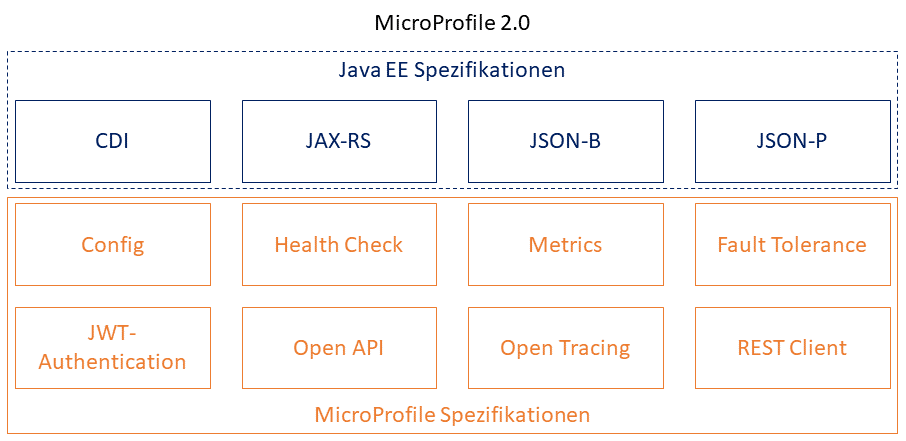
\includegraphics[width=\textwidth, center]{anhanga/microprofile_components}
	\caption[Beschreibung für Verzeichnis2]{Bildunterschrift2}
	\label{img:microprofile_components}
\end{figure}